% Hybrid level diagram for Section 3.
% Build:
%   pdflatex -output-directory=/tmp diagram-final.tex
%   cp /tmp/diagram-final.pdf ../../figs/approach-hybrid.pdf
\documentclass[tikz,border=4pt]{standalone}
\usepackage[T1]{fontenc}
\usetikzlibrary{arrows.meta,fit,backgrounds,shapes.geometric,calc}
\begin{document}
\sffamily\footnotesize
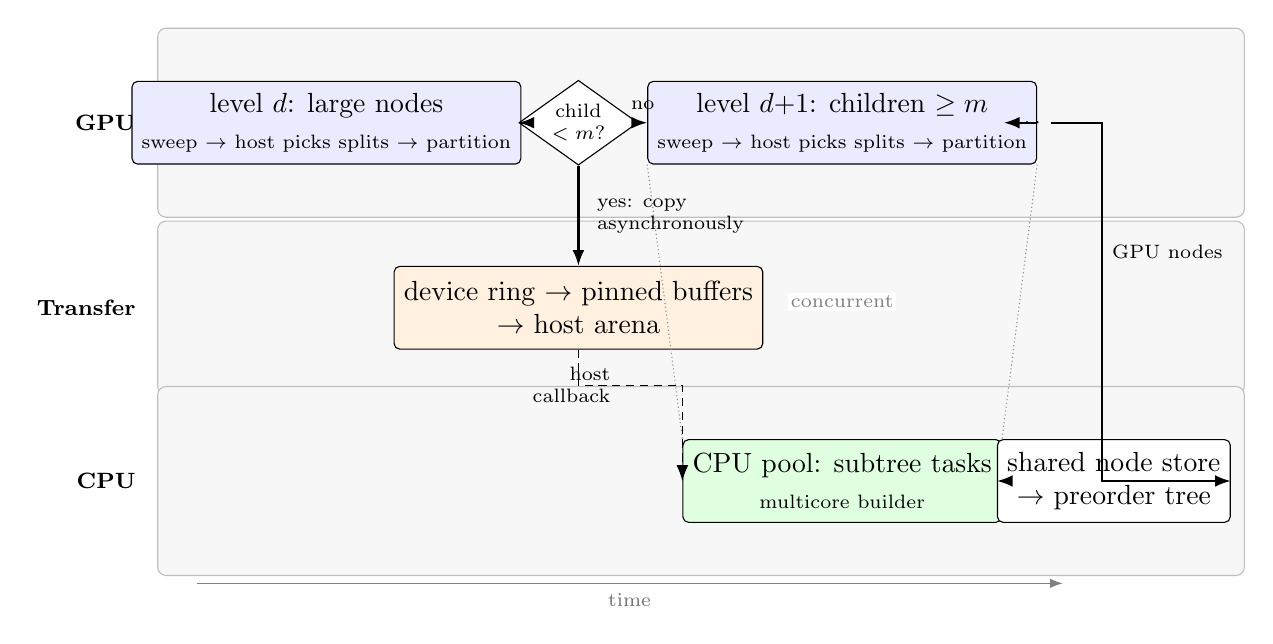
\begin{tikzpicture}[
  box/.style={draw, rounded corners=2pt, align=center, inner sep=3.5pt,
              minimum height=10.5mm},
  gpu/.style={box, fill=blue!8},
  xfer/.style={box, fill=orange!12},
  cpu/.style={box, fill=green!12},
  fork/.style={draw, diamond, aspect=1.4, inner sep=1pt, fill=white,
               align=center, font=\scriptsize, minimum width=14mm},
  flow/.style={-{Latex[length=2mm]}, thick},
  async/.style={-{Latex[length=2mm]}, densely dashed},
  lane/.style={draw=black!25, fill=black!3, rounded corners=3pt},
  lanelbl/.style={font=\bfseries\footnotesize, anchor=east},
  note/.style={font=\scriptsize, align=center}]

% Lane centres: y = 0 / -2.35 / -4.55. Extra left margin for labels.
\begin{scope}[on background layer]
  \node[lane, minimum height=24mm, minimum width=138mm, anchor=west]
    at (0.7,0) {};
  \node[lane, minimum height=22mm, minimum width=138mm, anchor=west]
    at (0.7,-2.35) {};
  \node[lane, minimum height=24mm, minimum width=138mm, anchor=west]
    at (0.7,-4.55) {};
\end{scope}
\node[lanelbl] at (0.55,0) {GPU};
\node[lanelbl] at (0.55,-2.35) {Transfer};
\node[lanelbl] at (0.55,-4.55) {CPU};

% GPU row (y=0), with room around the diamond.
\node[gpu, minimum width=35mm] (lvd) at (2.85,0)
  {level $d$: large nodes\\[1pt]
   \scriptsize sweep $\rightarrow$ host picks splits $\rightarrow$ partition};
\node[fork] (test) at (6.05,0) {child\\$<m$?};
\node[gpu, minimum width=35mm] (lvd1) at (9.4,0)
  {level $d{+}1$: children $\ge m$\\[1pt]
   \scriptsize sweep $\rightarrow$ host picks splits $\rightarrow$ partition};
\node[note] (more) at (11.75,0) {$\cdots$};

\draw[flow] (lvd) -- (test);
\draw[flow] (test) -- node[above, note, yshift=1pt] {no} (lvd1);
\draw[flow] (lvd1) -- (more);

% Transfer row (y=-2.35).
\node[xfer, minimum width=40mm] (arena) at (6.05,-2.35)
  {device ring $\rightarrow$ pinned buffers\\$\rightarrow$ host arena};
\draw[flow] (test) -- node[right, note, xshift=3pt, align=left]
  {yes: copy\\asynchronously} (arena);

% CPU row (y=-4.55).
\node[cpu, minimum width=40mm] (tasks) at (9.4,-4.55)
  {CPU pool: subtree tasks\\[1pt]
   \scriptsize multicore builder};
\node[box, fill=white, minimum width=28mm] (store) at (12.85,-4.55)
  {shared node store\\$\rightarrow$ preorder tree};

\draw[async] (arena.south) -- ++(0,-0.45) -|
  node[pos=0.2, left, note, align=right] {host\\callback} (tasks.west);

% Concurrent marker: short dotted braces + label between the two boxes.
\coordinate (cL) at ($(lvd1.south west)!0.5!(tasks.north west)$);
\coordinate (cR) at ($(lvd1.south east)!0.5!(tasks.north east)$);
\draw[black!45, densely dotted] (lvd1.south west) -- (tasks.north west);
\draw[black!45, densely dotted] (lvd1.south east) -- (tasks.north east);
\node[note, text=black!50, fill=white, inner sep=1pt]
  at ($(cL)!0.5!(cR)$) {concurrent};

\draw[flow] (tasks) -- (store);
% Clear right-side route from GPU continuation into the store.
\draw[flow] (more.east) -- ++(0.65,0) |- 
  node[pos=0.18, right, note] {GPU nodes} (store.east);

\draw[-{Latex[length=1.6mm]}, black!50]
  (1.2,-5.85) -- node[below, note, text=black!55] {time} (12.2,-5.85);
\end{tikzpicture}
\end{document}
